\chapter{Event Selection}
\label{event_selection_chapter}

This chapter details the requirements used to select events for the analysis.
It also covers the data used and the Monte Carlo (MC) used. The final state we
are considering is \Ztoee.

\section{Acceptance}

The acceptance region is a definition of what events, assuming that there are
no limitations due to the detector design, we include in our analysis. It is
essential to define an acceptance region so that our final result can be
compared to other measurements and to theory without forcing other groups to
attempt to correct for our experimental effects. The acceptance region defines
what sort of physics results we can make statements about, and also determines
the value of the effective cross-section of the \Z.

Our acceptance is defined by the kinematics of the two electrons and the mass
of the Z boson. One of the electrons, called the \CentralElectron, is required
to have $\pt > 30 \GeV$ and to be within the central region of the detector
(hence the name) with $|\eta| < 2.1$. The other electron, called the
\ExtendedElectron, has looser requirements; it must have $\pt > 20 \GeV$ and is
not required to be as central with $|\eta| < 2.4$. The requirements on the
\CentralElectron were selected in conjunction with the \Ztomumu measurement of
\phistar at CMS so that that measurement and this one could be easily combined
into a joint measurement. The pseudorapidity limit was selected to match the
most efficient region of CMS's single muon trigger, while the transverse
momentum threshold was dictated by threshold on single electron trigger. The
pseudorapidity limit on the \ExtendedElectron was chosen to keep all of the
electrons within the region covered by the tracker (which allows a better
angular measurement than ECAL alone), while the transverse momentum threshold
was selected because for $\pt < 20 \GeV$ the rate of fake electrons increases.

\begin{figure}[tb]
    \centering
    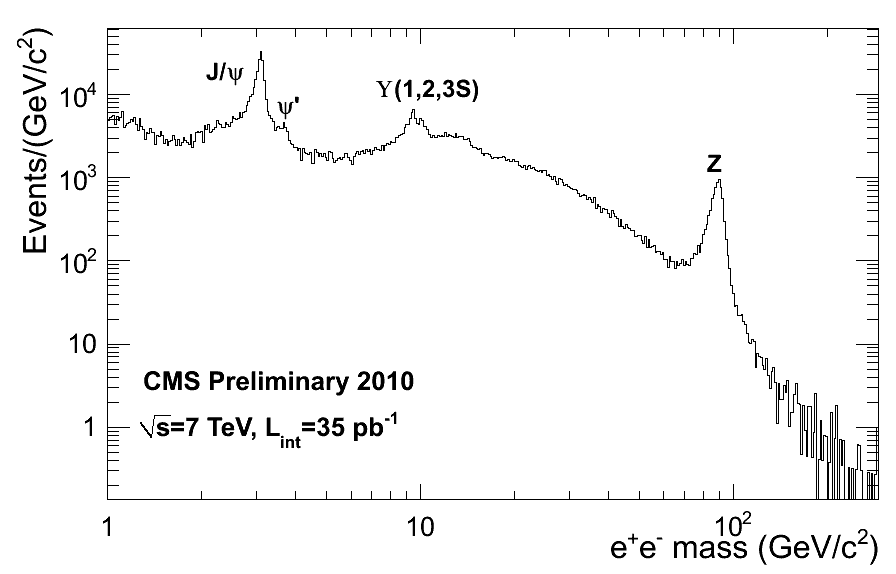
\includegraphics[width=\textwidth]{figures/dielectron_mass_7tev.png}
    \caption{The spectrum of \ee events as measured by CMS in 2010.}
    \label{fig:ee_spectrum}
\end{figure}

There are other particles, like the \jpsi, that decay to \ee pairs as shown in
\FIG~\ref{fig:ee_spectrum}. Fortunately, none of these other particles are near
the \Z in mass, and so we can eliminate them from our acceptance by requiring a
mass near the \Z peak. We therefore define our mass window around the nominal
\Z mass of $91 \GeV$, extending from $60 \GeV$ to $120 \GeV$.

\section{Data and Monte Carlo}

\subsection{Data}

The data used in this analysis were collected by the CMS detector in 2012 at a
center of mass energy of \rootseight. The LHC delivered 23 \fbinv of integrated
luminosity during the year as seen in \FIG~\ref{fig:2012_luminosity}. This
period was divided into four run eras called 2012A, B, C, and D. During an era,
the LHC run parameters are kept roughly static to allow for consistent data
taking conditions. In between eras, maintenance and minor upgrades are
performed on the LHC in order to deliver higher luminosity.

\begin{figure}[tb]
    \centering
    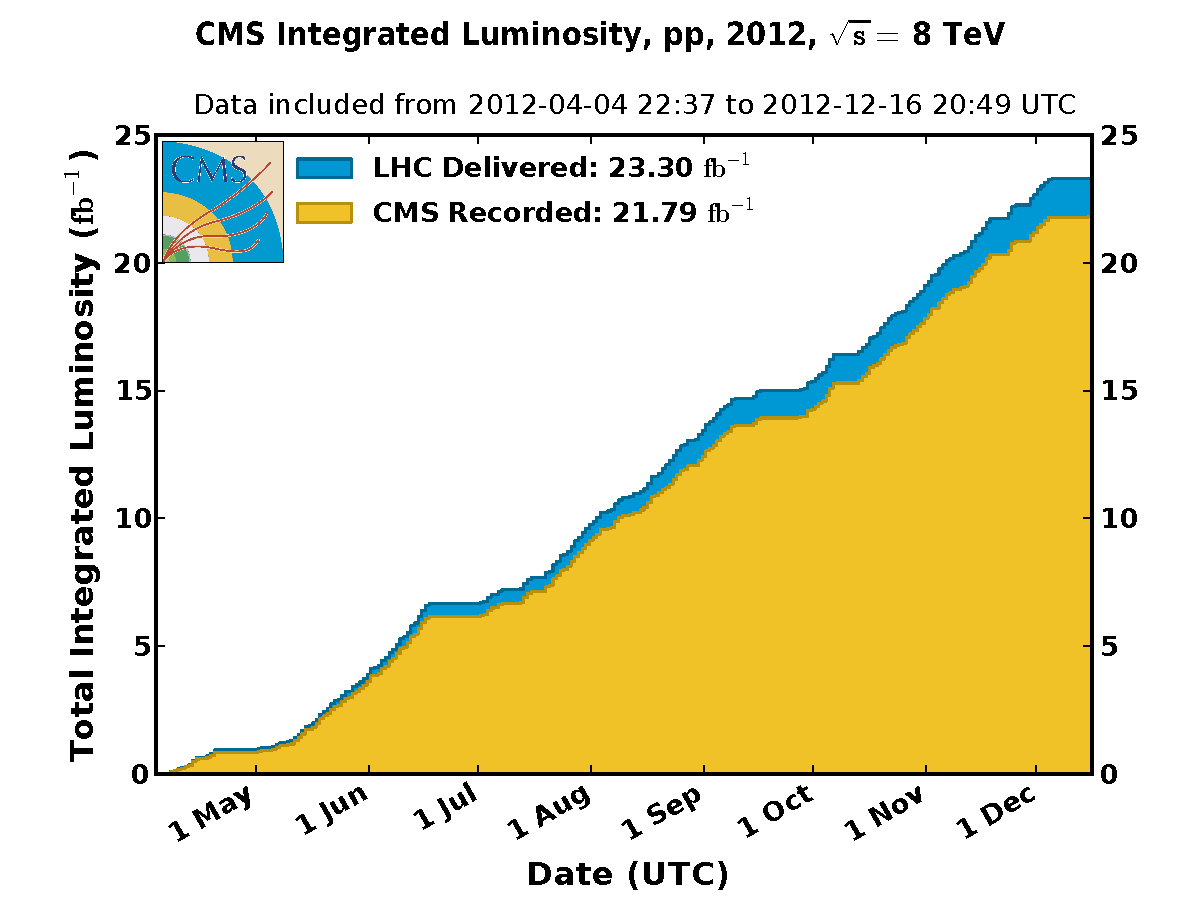
\includegraphics[width=\textwidth]{figures/2012_lumi.pdf}
    \caption{ The integrate luminosity per day delivered and recorded by CMS in
        2012. The flat periods in May, July, and September correspond to the
        boundaries between the run eras. }
    \label{fig:2012_luminosity}
\end{figure}

The data collected by CMS are split into smaller datasets based on the physics
objects contained within the events. This allows analyses to use only one or
two datasets, instead of requiring them to deal with the entirety of the CMS
data (which is petabyte scale, and hence too large for most institutes to store
locally). The HLT sorts events into the various datasets based on the triggers
that the event fired. In this manner, and event can end up in multiple datasets
if it fired multiple triggers. This analysis uses the \SingleElectron dataset
which was collected with the HLT trigger \SingleElectronTrigger. These datasets
were reconstructed---converted from raw detector response into physics
objects---in January, 2013, in order to make use of the most recent
calibrations derived from the entire 2012 run. A summary of the datasets used
are listed in \TAB~\ref{table:datasets}.

\begin{table}[h]
\centering
\begin{center}
    \begin{tabular}{ | l | c | c |}
    \hline
	Dataset Name                          & Run Range      & Luminosity       \\ \hline
	/SingleElectron/Run2012A-22Jan2013-v1 & 190456--193621 & $889.362 \pbinv$ \\ \hline
	/SingleElectron/Run2012B-22Jan2013-v1 & 193833--196531 & $4.429 \fbinv$   \\ \hline
	/SingleElectron/Run2012C-22Jan2013-v1 & 198022--203742 & $7.152 \fbinv$   \\ \hline
	/SingleElectron/Run2012D-22Jan2013-v1 & 203777--208686 & $7.318 \fbinv$   \\ \hline
    \end{tabular}
\end{center}
\caption{
    The datasets used in this analysis.
}
\label{table:datasets}
\end{table}

Although there is a \DoubleElectron dataset which uses a trigger designed to
find Z bosons, this analysis uses the \SingleElectron dataset selected with the
\SingleElectronTrigger trigger. The primary motivation behind using this
trigger was to allow a direct comparison with a similar \phistar analysis being
performed by CMS which used \Ztomumu events selected with a single muon
trigger. The single electron trigger requires an electron with $\pt > 27$ which
passes Working Point 80 (\WPEighty), a set of cuts on lepton isolation and
shower shape designed to be 80\% efficient on electrons. The cuts that make up
\WPEighty are listed in \TAB~\ref{table:wp80}. This trigger had the lowest \pt
threshold of any single electron trigger that was unprescaled run during 2012.
To prescale a trigger means to apply a rate reduction by randomly throwing out
a certain fraction of events in order to keep the total trigger rate
manageable; as this trigger was unprescaled, no events were discarded in this
manner.

\begin{table}[h]
\centering
\label{table:wp80}
\begin{center}
    \begin{tabular}{ | c | c | c |} \hline
        Value                      & EB     & EE     \\ \hline
        $|\eta| <$                 & 1.4791 & 2.65   \\
        $\pt >$                    & 27     & 27     \\
        $\sigmaietaieta <$         & 0.1    & 0.03   \\
        ECAL Iso $/ \et <$         & 0.15   & 0.1    \\
        $H/E <$                    & 0.1    & 0.05   \\
        HCAL Iso $/ \et <$         & 0.1    & 0.1    \\
        Pixel Matching $\ge$       & 1      & 1      \\
        $|\ooeoop| <$              & 0.05   & 0.05   \\
        $|\Delta \eta| <$          & 0.007  & 0.007  \\
        $|\Delta \phi| <$          & 0.06   & 0.03   \\ \hline
    \end{tabular}
\end{center}
\caption{
    The selection requirements for the \SingleElectronTrigger trigger for
    electrons which end up in the barrel region or the endcap region of ECAL.
}
\end{table}

\TODO{Put variables in an electron reconstruction chapter.}

The events from the \SingleElectron sample are further filtered for quality. A
centrally produced list of good luminosity segements is used to select only
events in which the part of the detector was malfunctioning or disabled. After
accounting for detector dead time and beam quality, \GoodLumiNumber of
integrated luminosity are used for physics analysis.
